\section{Antecedentes}

\begin{frame}
\frametitle{Tipos de galaxias}

\begin{center}
    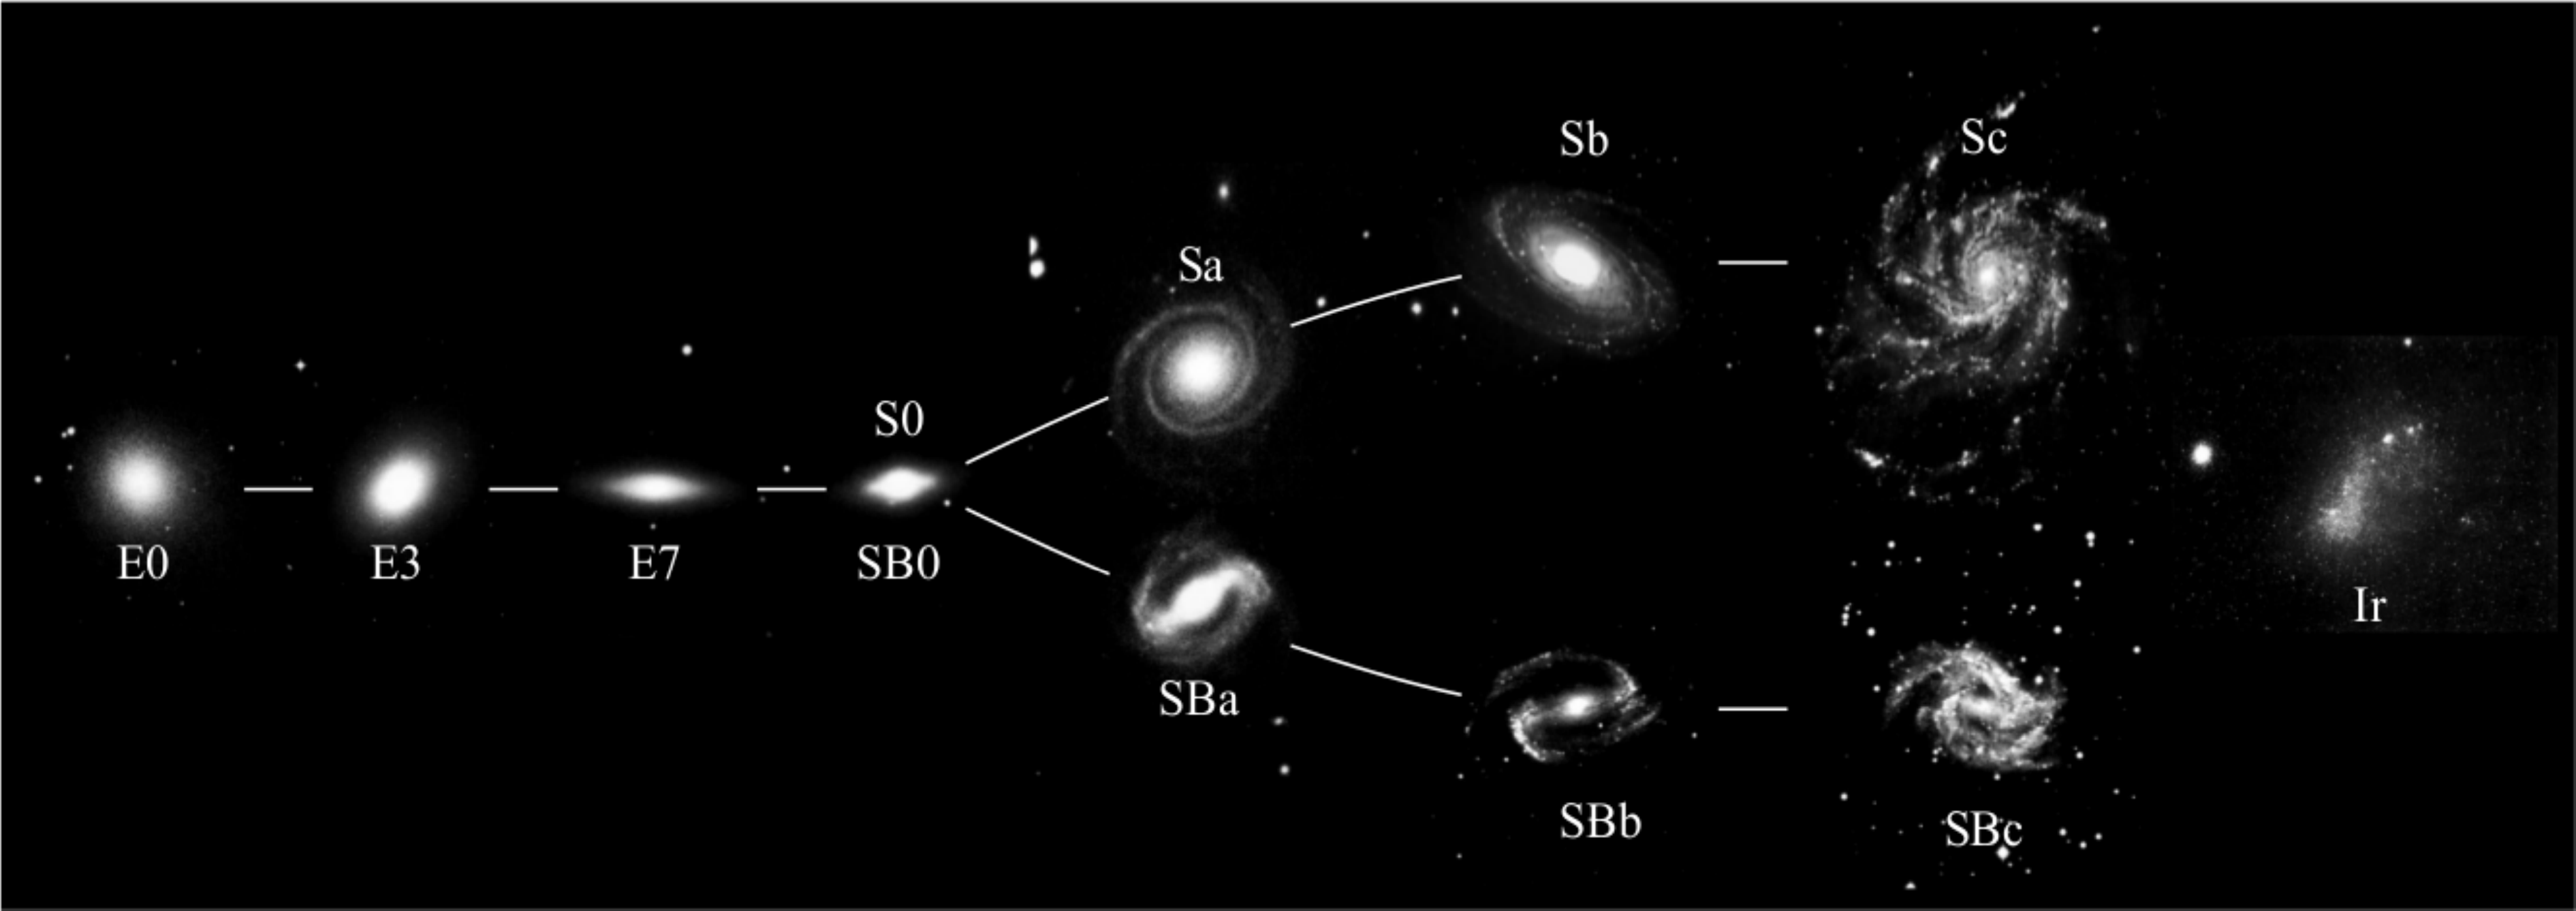
\includegraphics[width=12cm]{antecedentes/figures/hubble.png}
\end{center}

\begin{itemize}
\item Galaxias elípticas
\item Galaxias espirales
\end{itemize}

\note{
- Clasificacion morfologica o \textbf{secuencia de Hubble} \\
- galaxias elípticas (\textbf{E0-E7}) \\
- rama superior galaxias espirales sin barra \\
- rama inferior galaxias espirales con barra \\

}

\end{frame}

\begin{frame}
\frametitle{Componentes de una galaxia}

\begin{columns}
\column{0.3\textwidth}
\begin{center}
    \begin{itemize}
    \item Esferoide
    \begin{itemize}
        \item Bulge
        \item Halo
    \end{itemize}
    \item Disco
    \begin{itemize}
        \item Disco delgado
        \item Disco grueso
    \end{itemize}
\end{itemize}
\end{center}
\column{0.7\textwidth}
\begin{center}
    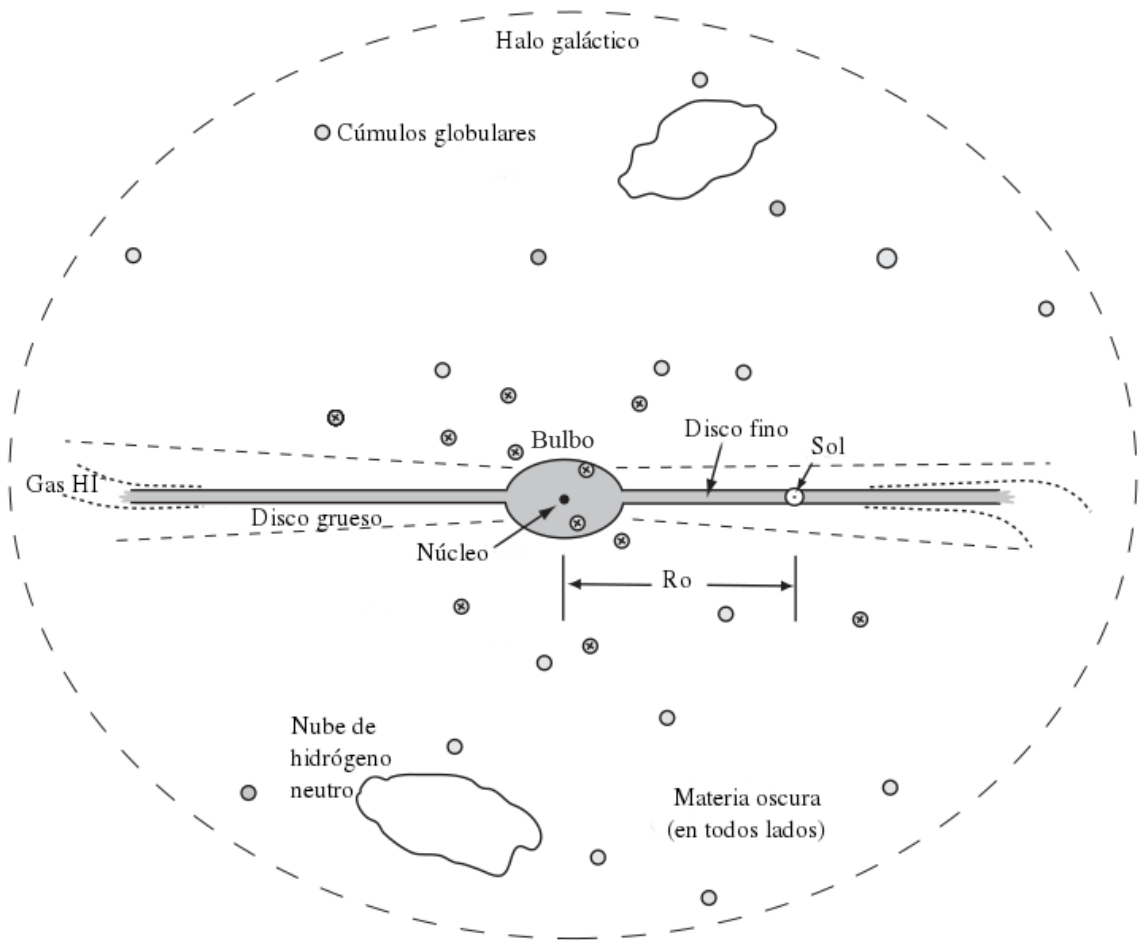
\includegraphics[width=8cm]{antecedentes/figures/mwschema.png}
\end{center}
\end{columns}

\note{
%\begin{itemize}
%\item Esferoide:
%    \begin{itemize}
%    \item Compuesto por una población estelar \textbf{roja} y vieja
%    \item Desde el punto de vista dinámico, las \textbf{estrellas del esferoide se encuentran soportadas por dispersión de velocidades, aunque puede presentar una rotación mínima}.
%    \item Subdivision
%    \end{itemize}
%\item Disco: 
%    \begin{itemize}
%    \item Compuesto principalmente por estrellas jóvenes, gas y polvo
%    \item Este es la componente principal de las galaxias espirales y lenticulares en lo que respecta a su masa.
%    \item Presenta una mayor tasa de formación estelar respecto al esferoide, debido a la existencia de gas en forma de hidrógeno, resultando en un color más azul gracias a la presencia de estrellas jóvenes
%    \end{itemize}
%\end{itemize}
}

\end{frame}




\begin{frame}
\frametitle{Problema observacional}

% 2.2.1 problemas de observacion al ver estrellas en x, y, z se puede confundir

\begin{center}
    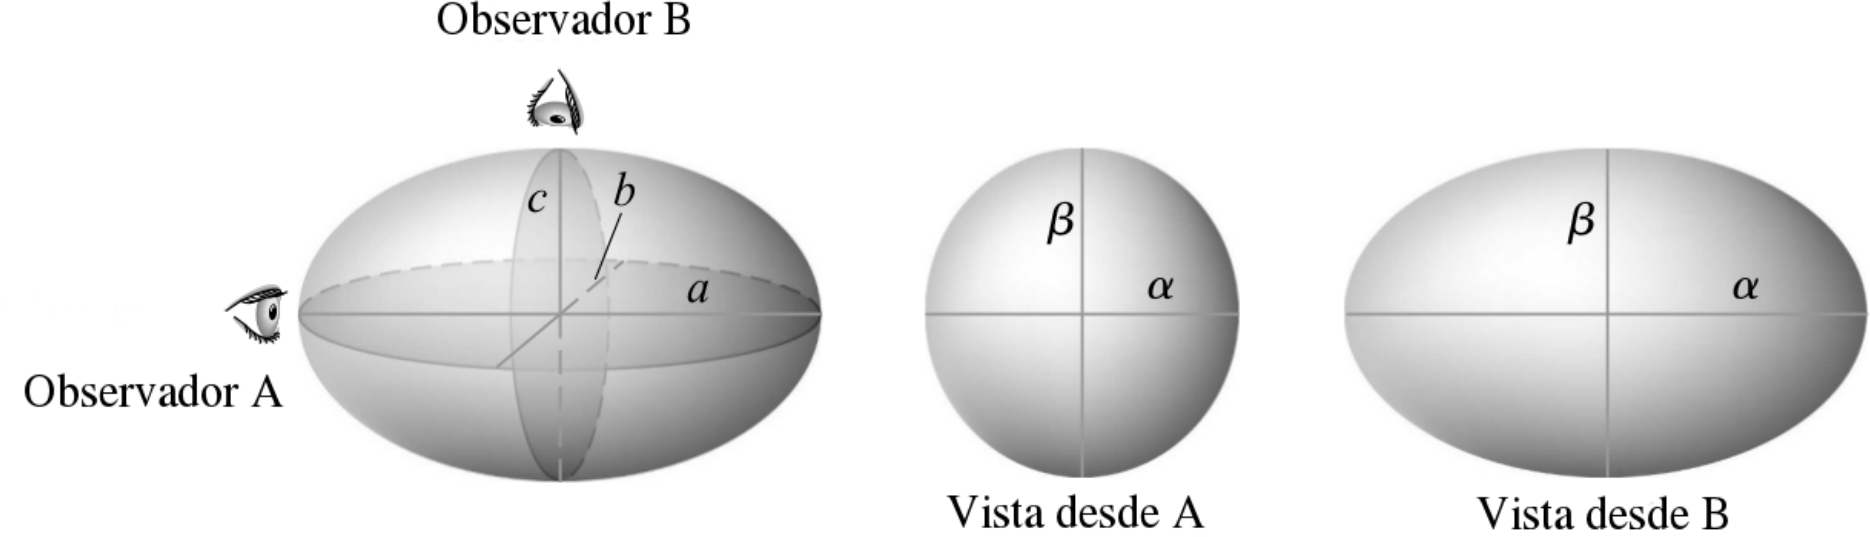
\includegraphics[width=12cm]{antecedentes/figures/proyecione_galactica.png}
\end{center}

\note{
\begin{itemize}
%\item Una galaxia elíptica con semiejes $a > b = c$,  observadores diferentes situados en diferentes posiciones percibirán diferentes formas proyectadas de este objeto, y consecuentemente la \textbf{clasificación} de particulas estelares \textbf{variará en cada caso}.
\item Problema en una proyección una estrella podría parecer que está en el esferoide mientras que \textbf{en realidad está en el disco}.
\item El area ha enfocado sus \textbf{esfuerzos en las características dinámicas de estrellas} en las componentes
%\item Requerimos de disponer de las posiciones y velocidades de las estrellas individuales que la conforman
%   \begin{itemize}
%    \item excede capacidades de telescopios actuales, por eso simulaciones
%    \end{itemize}
\item Estas caracteristicas (posiciones y velocidades de estrellas) no se pueden obtener con \textbf{telescopios actuales}, por lo cual \textbf{recurrimos a las simulaciones}
\end{itemize}
}

\end{frame}



\begin{frame}
\frametitle{Simulaciones}

\begin{center}
    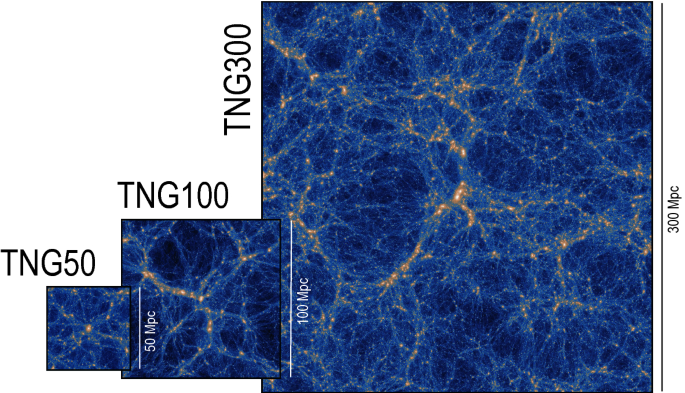
\includegraphics[width=12cm]{antecedentes/figures/tng.png}
\end{center}

\note{
- Estas simulaciones nos brindan la posibilidad de acceder a esta información. \\
- Estado del arte %en cuanto a combinar una alta resolución numérica con volúmenes computacionales cosmológicos suficientemente grande para que incluyan decenas de miles de galaxias individuales.
}

\end{frame}



\begin{frame}
\frametitle{Parámetros}

\begin{itemize}
    \item<2-> Parámetro de circularidad ($eps$):
        \[\epsilon = \frac{J_{z}(E)}{J_{circ}(E)}\]
    \item<3-> Parámetro de circularidad proyectada ($eps\_r$):
    \[\epsilon_{r} = \frac{J_{p}(E)}{J_{circ}(E)}\] Donde $J_P = \sqrt{J_x^2 + J_y^2}$
        
    \item<4-> Energía estelar normalizada ($normalized\_star\_energy$):
        \\
        \begin{center}
            $E/|E|_{max}$
        \end{center}
\end{itemize}

\note{
\begin{itemize}
\item<1-> Así, los tres valores que representan los movimientos de una partícula estelar y definen su ubicación en alguna de las componentes son \\
\item<2-> eps: Cuán \textbf{parecida} es la órbita de una partícula respecto a una \textbf{órbita circular}, para un dado valor de energía. %Es el cociente entre la componente z del \textbf{momento angular} y el momento angular que tendría una partícula, si utilizase toda su energía cinética para moverse en una órbita circular. \\
\item<3-> eps\_r: Representa la \textbf{dispersión vertical} del movimiento de una partícula con respecto al \textbf{plano} en el que se ubican las \textbf{partículas} que se mueven en \textbf{órbitas circulares}. %Donde $J_x$ y $J_y$ son las componentes restantes del vector momento angular de la partícula estelar. \\
\item<4-> norm: \textbf{que tan ligada} esta la particula a la galaxia%Cociente entre los valores de energía de las partículas estelares y el módulo de la energía de la partícula más ligada de la galaxia. \\
\item<4-> Las partículas más ligadas al sistema van a adoptar valores cercanos a -1, mientras que las menos ligadas van a  tener valores cercanos a 0.
\end{itemize}
}

\end{frame}



\begin{frame}
\frametitle{Métodos Establecidos}

\begin{itemize}
    \item Abadi
    \item Auto-Gaussian Mixture Model (AGMM)
\end{itemize}

\begin{center}
    
\includegraphics[width=12cm]{antecedentes/figures/galaxychop_logo.png}
    \href{https://github.com/vcristiani/galaxy-chop}{https://github.com/vcristiani/galaxy-chop}
\end{center}

\note{
- Abadi: Usa \textbf{eps} para separar en \textbf{Disco} y \textbf{Esferoide}. Asume que la componente esferoidal no presenta rotación y por lo tanto está representada por una distribución simétrica respecto de $\epsilon = 0$. Para ello selecciona el mismo número de partículas en órbitas corrotantes que aquellas que se encuentran en órbitas contrarrotantes. Luego, la distribución de las partículas restantes, se asignará al disco. Esto se debe a que el método asume que el disco está formado por partículas cuyo movimiento predominante es el de rotación. Como reflejo de esto, las partículas asignadas al disco tendrán $\epsilon \sim 1$. \\
- AGMM: Realiza \textbf{distribuciones Gaussianas} que representan las estructuras a ser identificadas, utilizando \textbf{$eps$, $eps_r$ y $normalized_star_energy$}. Genera dichos modelos variando el \textbf{número de componentes a buscar de 2 a 9}. En cada iteración, se crean 10 modelos con diferentes inicializaciones para alcanzar resultados más estables. El algoritmo usa una función a minimizar y un valor de disparo previamente establecido. Como la iteración comienza con 2 grupos y crece desde ahí, se tiene preferencia en buscar pocas componentes.
}

\end{frame}

\iflong
\begin{frame}
\frametitle{Aprendizaje automático}
\centering ¿Que es Machine Learning?

\pause

\vspace{0.5cm}

\begin{displayquote}
\textit{Se dice que un programa de computadora aprende de la experiencia $E$
respecto a una tarea $T$ y una medida de desempeño $P$, si el desempeño medido con $P$ en una tarea $T$, mejora con la experiencia $E$.}
\end{displayquote}

\note{
- La \gls{AI} tiene diferentes ramas siendo la de éxito actual aquella que postula que se puede imitar la inteligencia humana por medio del aprendizaje. En otras palabras, podemos brindar datos de ejemplo a un programa para que entienda su ``forma'' y generalice en una tarea dada. \\
- El \gls{ML} es un proceso inductivo para la exploración de conocimiento, donde su enfoque reside en la búsqueda de información general a partir de observaciones específicas que sesgan las suposiciones de conocimiento concreto, con el propósito de establecer una base sólida para realizar generalizaciones. 
}

\end{frame}
\fi


\iflong
\begin{frame}
\frametitle{Tipos de Aprendizaje Automático}

\begin{itemize}
    \item<1-> Aprendizaje Supervisado
    \item<2-> Aprendizaje No-Supervisado
\end{itemize}

\note{
%- Todos los métodos de \gls{ML} requieren datos de entrenamiento para adquirir conocimiento. Sin embargo, diversos tipos de tareas ($T$), experiencias ($E$) y desempeños ($P$) conducen a múltiples especializaciones. La clasificación inicial más común categoriza a los modelos de \gls{ML} en función de cómo el algoritmo utiliza o no valores objetivos a aproximar: \\
%- Supervisado: Aproxima la función $F(X) = y$, con $X$ como datos de entrada o matriz de \textit{features} y el vector $y$ corresponde a sus respectivas etiquetas o clases objetivos. Puede tomar la forma de un conjunto finito de etiquetas discretas (clasificación) o intentar predecir un valor numérico real que represente alguna magnitud (regresión). \\
- Supervisado: Utiliza un \textbf{conjunto de entrada y salidas} para entrenar un \textbf{modelo} que se usara para predecir nuevas entradas. \\
- No supervisado: Adquiere conocimiento durante la ejecución de la tarea sin requerir etiquetas. \\%Ej reducción de la dimensionalidad, la visualización de datos (manteniendo sus propiedades fundamentales) o la agrupación en conjuntos con características similares. \\
%- Dos etapas: la de entrenamiento y la de predicción. Además, hay varios modelos que poseen hiperparámetros que pueden ser configurados previamente a la fase de entrenamiento. \\
- Falta de etiquetas en galaxias, vamos a hacer no supervisado
}

\end{frame}
\fi

\begin{frame}
\frametitle{Metodos de Clustering}

\begin{itemize}
    \item<2-> Métodos jerárquicos
    \item<3-> Métodos difusos/\textit{fuzzy}
    \item<4-> Métodos basados en acumulación de evidencia
\end{itemize}

\note{
\begin{itemize}
\item<1-1> Utilizaremos entonces metodos de Clustering (que son no-supervisados) para asignar las partículas estelares a las diferentes componentes galácticas. Los algoritmos de \textit{clustering} tienen la \textbf{tarea de agrupar un conjunto de objetos} de tal manera que los objetos de un mismo grupo (llamado \textit{cluster}) sean \textbf{más similares}, en algún sentido, entre sí \textbf{que los de otros} grupos ($clusters$). \\
\item<2-> Jerarquico: Crean agrupamientos basándose en agrupamientos más pequeños de una manera jerárquica. Buscamos reflejar\textbf{ estructura jerarquica de galaxia}. \\
\item<3-> Fuzzy: Dado que una partícula de varias masas solares \textbf{puede pertenecer a más de una componente} galáctica al mismo tiempo, queremos evaluar cómo se comporta los métodos de agrupamientos basados en \textbf{lógica difusa} para la asignación de la misma partícula en diferentes componentes. \\
\item<4-> EAC: Permiten \textbf{combinar y consensuar} resultados provenientes de otras técnicas de clustering. Para \textbf{busacar estructuras complejas} que no son posibles de encontrar en un solo metodo de agrupamiento.
\end{itemize}
}

\end{frame}






%saltear rapido
\begin{frame}
\frametitle{Métricas de validación externa}

\begin{columns}
\column{0.45\textwidth}
\begin{center}
    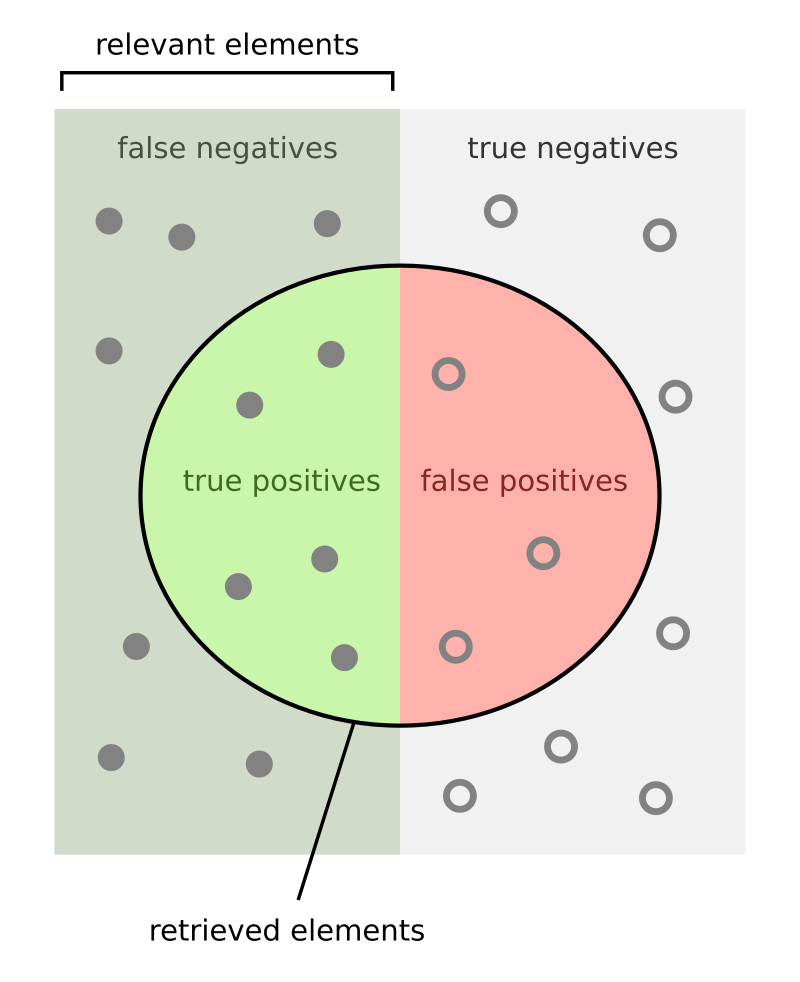
\includegraphics[width=6cm]{antecedentes/figures/Precisionrecall-1.png}
\end{center}
\column{0.7\textwidth}
\begin{center}
    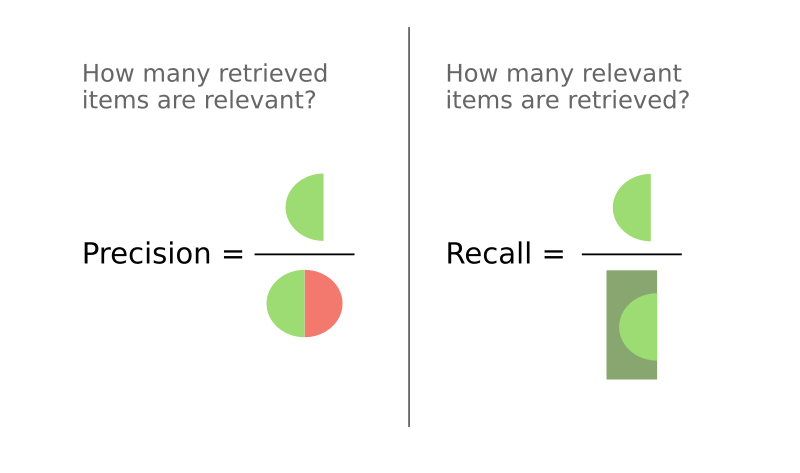
\includegraphics[width=8cm]{antecedentes/figures/Precisionrecall-2.png}
\end{center}
\end{columns}

%\begin{itemize}
%    \item<1-> Presicion
%    $$Precision = \frac{TP}{TP + FP}$$
%    \item<2-> Recall
%    $$Recall = \frac{TP}{TP + FN}$$
%\end{itemize}

%\begin{table}[]
%    \centering
%    \begin{tabular}{c|c|c}
%         {}                   & \multicolumn{2}{l}{\textbf{Clase Predicha}} \\
%         \textbf{Clase Real}  & \textbf{Positiva}  &  \textbf{Negativa}                        \\
%         \textbf{Positiva }            &  \gls{TP}       & \gls{FN}                               \\
%         \textbf{Negativa}             &  \gls{FP}       & \gls{TN}
%    \end{tabular}
%\end{table}

\note{
\begin{itemize}
\item Clustering \textbf{discierne grupos entre sí}, no los cataloga. Una vez \textbf{etiquetados los datos manualmente}, es necesario \textbf{compararlos} con los obtenidos con algún método que tengan una fundamentación física sólida y además provean estas etiquetas. Los resultados de estos metodos los llamaremos GT, y vendran de \textbf{Abadi} y \textbf{AGMM}. Teniendo el cuidado de utilizar los mismos parámetros dinámicos en cada caso. %Comparando los resultados de \gls{GT} y los del metodo a evluar, podemos crear la \gls{CM} (explicar con dos clases). 
\item Presicion:  Cuánto de lo que seleccioné era realmente relevante.  %La proporción de partículas bien asignadas a una componente respecto al total que fue asignada a esa componente. \\
\item Recall: Cuánto de lo relevante fue seleccionado. %La proporción de partículas bien asignadas a una componente respecto al total que debería haber sido asignado a esa componente.  \\
%\item Hacer \textbf{promedio pesado} para aplicar a todas las clases y lidiar con el desbalance de clases (ej flores?)
\end{itemize}
}

\end{frame}



\begin{frame}
\frametitle{Métricas de validación interna}

\begin{itemize}
    \item<1-> Puntaje de Silhouette (SSc)
    $$
    s(i)={\frac {b(i)-a(i)}{\max\{a(i), b(i)\}}}
    $$
    \begin{itemize}
    \item $a(i)$: promedio de la distancia entre el punto $i$ con todos los puntos del mismo cluster
    \item $b(i)$: promedio de la distancia entre el punto $i$ con todos los puntos del cluster más cercano
    \end{itemize}
    \item<2-> Índice de Davies–Bouldin (DBI) \\
    Busca para todos los \textit{clusters} $c_i$, el \textit{cluster} $c_j$ que maximiza el valor $R_{ij}$, para luego promediar todos los valores $R_{ij}$ obtenidos. 
    \begin{itemize}
        \item $s_i$: La distancia promedio de cada punto en el \textit{cluster} $c_i$ al centro de su mismo \textit{cluster}
        \item $d_{ij}$: Distancia entre los centros de los \textit{clusters} $c_i$ y $c_j$
        \item $R_{ij}$: La suma de $s_i$ y $s_j$ dividido $d_{ij}$
    \end{itemize}
\end{itemize}

\note{
- Utilizan todo el conjunto de datos que se usó para entrenar al modelo, y analizan la \textbf{distancia intra y extra \textit{cluster}}, y la continuidad espacial que tienen los datos dentro de sus clusters. Esto da una idea de la estructura interna sin necesidad de recurrir a valores externos. \\
- Silhouette: El puntaje es el promedio del coeficiente en cada punto. Valores $\sim 1$ \textit{clusters} están bien separados entre si y son a su vez bien compactos; valores $\sim -1$ existen puntos mal clasificados; $\sim 0$ existe una superposición entre \textit{clusters} \\
- Davies Bouldin: Valores $\sim 0$ mejor agrupamiento, valores alejados de $0$ (hasta infinito) dan a entender un mal trabajo de \textit{clustering}. \\
- Valores \textbf{alejados del ideal} no esta necesariamente mal, depende de la \textbf{naturaleza de los clusters}
}

\end{frame}








\begin{frame}
\frametitle{Análisis físicos del área}

Curva de Perfil de Velocidades
\begin{center}
    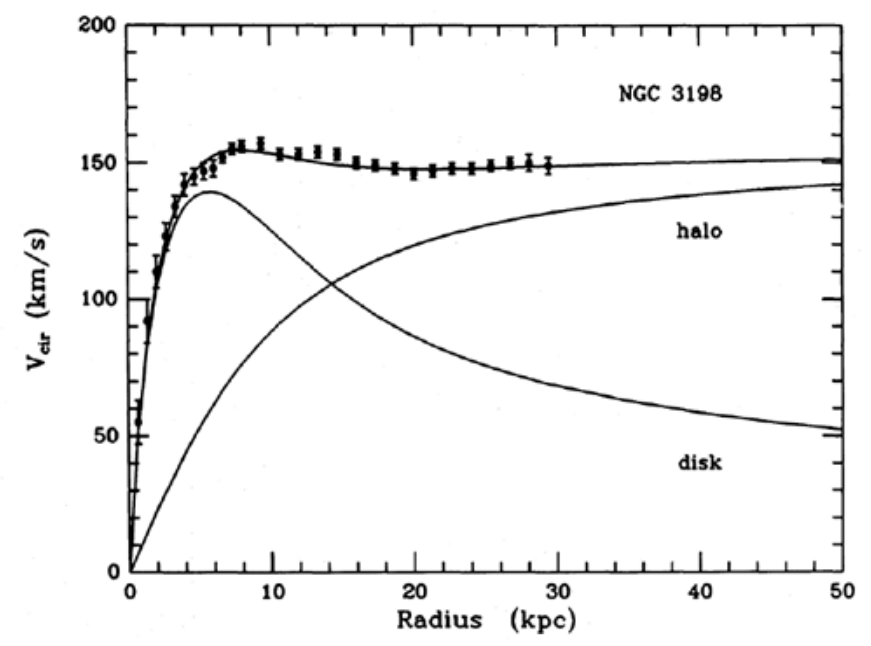
\includegraphics[width=8cm]{antecedentes/figures/vprofile.png}
\end{center}

\note{
%- Crear un puente hacia los astrónomos presentando los resultados en una forma que es habitual en el área. \\
%- Hay otras mas complejas, asi que usamos esta simple que podemos entender \\
- Muestran la \textbf{velocidad de rotación} de las componentes en una galaxia en función de su \textbf{distancia radial al centro} de las mismas. \\
%- por ej, las estrellas del disco se acumulan más cerca del centro de la galaxia, mientras que las partículas del halo predominan en la región más externa de la misma. Esperable para dichas componentes. \\
- Si \textbf{superponemos nuestras curvas} con \gls{GT}, ver si en la dinámica de las componentes identificadas se reproducen los comportamientos típicos estudiados en la física; esto lo vuelve una \textbf{métrica externa}.
}

\end{frame}




\begin{frame}
\frametitle{Remover Atípicos/Outliers}

\begin{itemize}
    \item<2-> Isolation Forest
    \begin{center}
        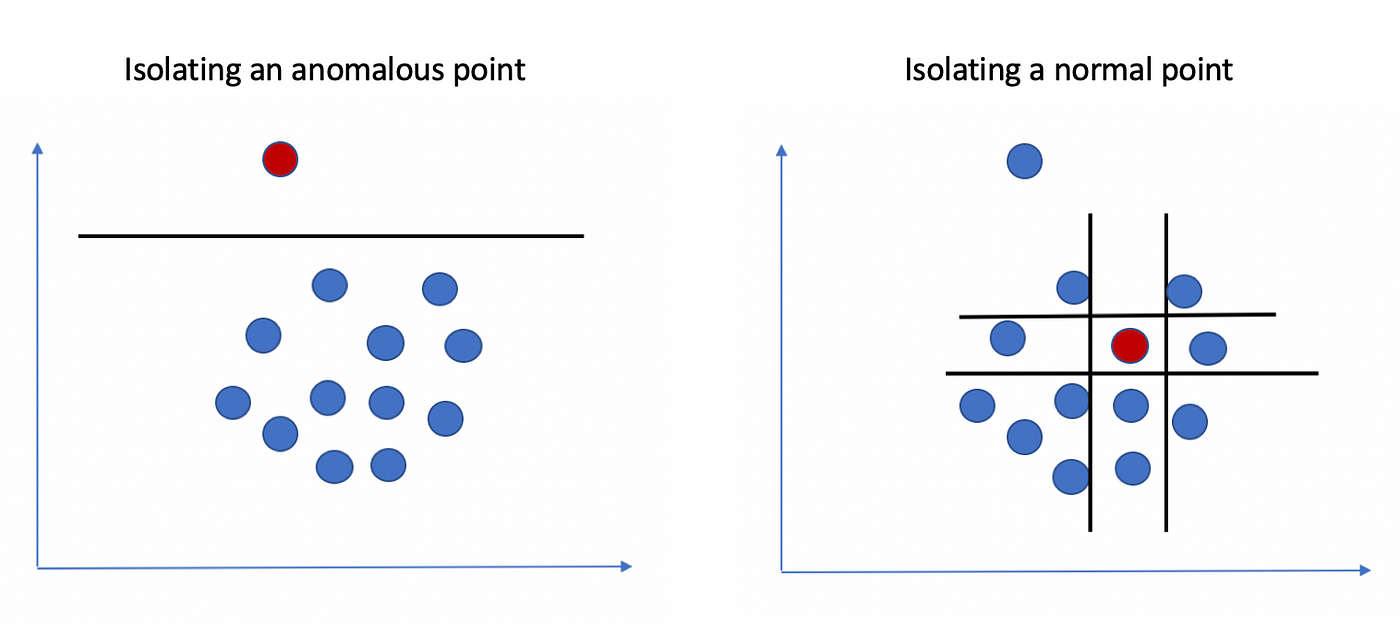
\includegraphics[width=8cm]{antecedentes/figures/isolation_forest.png}
    \end{center}
    \item<3-> RCut
\end{itemize}

\note{
\begin{itemize}
\item<1-> Podemos considerar atípicos a valores que están muy \textbf{alejados del centro galáctico} y puede que estén muy \textbf{débilmente ligados gravitacionalmente}
\item<2-> IF: Detecta anomalías mediante árboles binarios. Divide el espacio de datos mediante \textbf{líneas paralelas a la base canónica} y asigna puntuaciones de anomalía a los datos, con valores más altos a los puntos de datos que necesitan menos divisiones para ser aislados. %Para aislar un punto del resto de los datos, el algoritmo genera recursivamente particiones en la muestra seleccionando aleatoriamente un atributo, para luego seleccionar también de forma aleatoria un valor de partición entre los valores mínimo y máximo permitidos por ese atributo. Aplicado sobre las coordenadas en el espacio real de cada partícula estelar, en lugar de utilizar los parámetros de circularidad descritos anteriormente.
\item<3-> RCut: Desde el punto de vista de la astrofísica, es habitual considerar a las galaxias como las partículas estelares con radio $r <= X Kpc$, donde $X$ es 3 veces el radio que encierra la mitad de la masa estelar. Esta heurística es usada en diversos trabajos como una \textbf{forma rápida de descartar valores} que es poco probable que pertenezcan a la galaxia, pero que el algoritmo que identifica las galaxias las haya asignado allí.
\end{itemize}
}

\end{frame}



\begin{frame}
\frametitle{Recursos computacionales}

Recursos computacionales proveídos por:

\begin{columns}
\column{0.5\textwidth}
\begin{center}
    
\includegraphics[width=6cm]{antecedentes/figures/IATE-01.png}
\end{center}
\column{0.5\textwidth}
\begin{center}
    
\includegraphics[width=6cm]{antecedentes/figures/ccad_solo_new.png}
\end{center}
\end{columns}

\begin{center}
    
\includegraphics[width=6cm]{antecedentes/figures/cenits.jpg}
\end{center}

\note{
- Algoritmos son \textbf{caros computacionalmente y en memoria} con la gran cantidad de datos que analizamos, por lo cual requerimos de supercomputadoras para correrlos. \\
- \textbf{Instituto de Astronomía Teórica y Experimental}, y el \textbf{Centro de computacion de alto desempeño} de la Universidad Nacional de Córdoba \\
- \textbf{Centro Extremeño de Investigación, Innovación Tecnológica y Supercomputación}, que forman parte de la Fundación Computación y Tecnologías Avanzadas de Extremadura de la \textbf{Red Española de Supercomputación}.
}

\end{frame}
